\documentclass{article}


% If you need to pass options to natbib, use, e.g.:
%     \PassOptionsToPackage{numbers, compress}{natbib}
% before loading neurips_2023


% ready for submission
\usepackage[final]{neurips_2023}
\usepackage{amsmath}
\usepackage{graphicx}
\usepackage{float}
\usepackage{subfig}         % display sub-figure
\usepackage[utf8]{inputenc} % allow utf-8 input
\usepackage[T1]{fontenc}    % use 8-bit T1 fonts
\usepackage{hyperref}       % hyperlinks
\usepackage{url}            % simple URL typesetting
\usepackage{booktabs}       % professional-quality tables
\usepackage{amsfonts}       % blackboard math symbols
\usepackage{nicefrac}       % compact symbols for 1/2, etc.
\usepackage{microtype}      % microtypography
\usepackage{xcolor}         % colors

\title{Dynamic Daytime Simulation with Snow Effect}

% The \author macro works with any number of authors. There are two commands
% used to separate the names and addresses of multiple authors: \And and \AND.
%
% Using \And between authors leaves it to LaTeX to determine where to break the
% lines. Using \AND forces a line break at that point. So, if LaTeX puts 3 of 4
% authors names on the first line, and the last on the second line, try using
% \AND instead of \And before the third author name.


\author{%
  Steven Webb\\\\
  u7544998 
   \And
  Mike Blue\\\\
  u333333\\
  \AND  The Australian National University 
}

\begin{document}

\maketitle


\begin{abstract}
  In order to preserve structural edges and shapes while simplifying the triangle mesh of man-made 3D models, we propose a new quadric error metric based on the distances between the new vertex position and the affected edges for edge collapse operations. With a 2D view sampling method, the contour and silhouette likelihood of the edges are computed, which act as the quadric’s weights during the mesh decimation. The comparisons and analysis among our methods with different weighting schemes will be presented in this report. We also compare our method with QSlim  and structure-aware mesh decimation method in multiple cases. Output generated by our method is better than QSlim and comparable to structure-aware method in most of the cases. 
\end{abstract}


\section{Introduction}

%For our final project, we implemented a system for rendering forests of trees in real time. We are using the method outlined in Eric Bruneton and Fabrice Neyret’s Real-time Realistic Rendering and Lighting of Forests[1], specifically their z-field method for rendering trees of apparent sizes larger than a few pixels. Trees are often difficult to render in real-time applications as their geometry is complex, though simplified methods are easy to identify as lower quality. Our program provides fast and accurate rendering of trees as well as a fractal based landscape to simulate a forest. In this paper, we explain the motivation for this model, then describe the algorithms used. We finish up with some ideas for future work and some of the bugs we encountered.

%Please read the instructions below carefully and follow them faithfully. 


\section{Motivation and Problem Statement}

%Trees are often a plentiful part of landscapes, and so rendering them at the same level of fidelity as foreground objects can make real-time rendering impossible. At the same time, lower fidelity objects can detract from a scene’s appearance, even if they are part of the background.
%# 1
% Moderate-quality tree models can be 250,000 or more triangles[2]. Just 20 of such trees would involve 5 million polygons. For comparison, a frame in the 2007 game Lost Planet can have 3 million polygons in a frame. Clearly, conventional rendering methods do not permit the use of such tree models in games. Games must instead rely on include low quality tree models or other workarounds of reduced fidelity.
%Bruneton and Fabrice [1] implemented a fast means of rendering high quality mid-distance trees, display- ing 180,000 such trees at over 30 frames per second. We hoped to duplicate their success, rendering tens of thousands of trees across a landscape in real time.
%Papers to be submitted to NeurIPS 2023 must be prepared according to the
%instructions presented here. Papers may only be up to {\bf nine} pages long,
%including figures. Additional pages \emph{containing only acknowledgments and
%references} are allowed. Papers that exceed the page limit will not be
%reviewed, or in any other way considered for presentation at the conference.
%
%
%The margins in 2023 are the same as those in previous years.
%%
%
%Authors are required to use the NeurIPS \LaTeX{} style files obtainable at the
%NeurIPS website as indicated below. Please make sure you use the current files
%and not previous versions. Tweaking the style files may be grounds for
%rejection.
%

\section{Previous Works}
% The ground under the trees is dynamically generated at runtime when the program is run. The diamond- square method of fractal terrain generation is used to create a height map, which is then applied to a square grid to create varied terrain. Points are set to the average height of particular surrounding points, then a random offset is added for variation. The offset is generated uniformly at random on the range (−x, x), where x is set before the algorithm is run, and is reduced by 2−y each iteration, where y can be adjusted. x is directly related to the maximum and minimum heights produced, and y is inversely related to the steepness of generated terrain. Lengths in the algorithm are the number of points between the current point and the other point in consideration, and can only be considered in horizontal or vertical lines. Points which are adjacent form a line of length zero. The diamond-square method in pseudocode [3] follows. 

\section {Methods and Algorithms}

%  Snow method 1: Color
\subsection {Snow Rendering}
TODO: Snow Rendering and CG algorithms

\subsubsection {Snow Color Function}

\subsubsection {Snow Accumulation Prediction Function}
Assume there is no wind in the scene, so all snow will fall vertically. The snow amount on a point can be 
determined by an exposure function, an inclination function, and a user-defined function.

The exposure function \( f_{e}(p) \) to calculate the occlusion that prevents snow from falling on the surface. % TODO: REF
\( f_{e}(p) \in (0, 1] \). \( f_{e}(p)=0 \) means that the point is fully occluded by another object, which is right 
above it, so there are no snowing effects on this point. \( f_{e}(p)=1 \) means that the point is exposed to the falling
snow. This function is based on a shadow map by setting a virtual directional light right above the object. The light 
direction is to the ground, so the points in the virtual shadow are also occluded by another object. Besides, to make
the transition process smoother, soft shadowing techniques can be used.

%\begin{figure}[h]
%  \centering
%  \subfloat[Snow Amount = 0.0]{
%    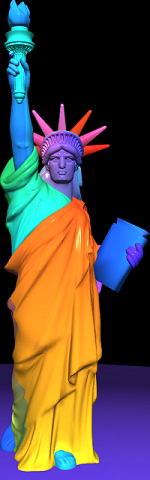
\includegraphics[width=0.30\textwidth]{images/AllTimeNaNNoSnow.png}
%    \label{fig:AllTimeNaNNoSnow}
%  }\hfill
%  \subfloat[Snow Amount = 0.5]{
%    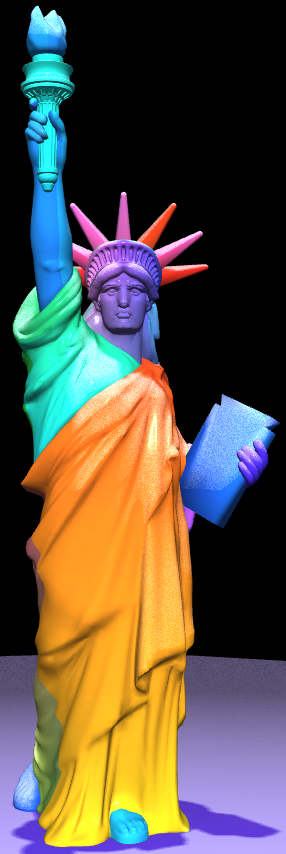
\includegraphics[width=0.30\textwidth]{images/AllTimeNaNHalfSnow.png}
%    \label{fig:AllTimeNaNHalfSnow}
%  }\hfill
%  \subfloat[Snow Amount = 1.0]{
%    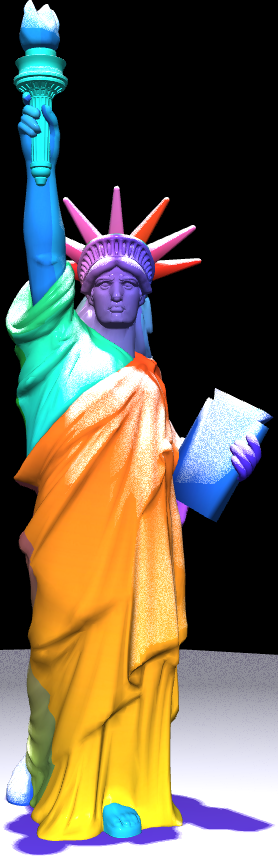
\includegraphics[width=0.30\textwidth]{images/AllTimeNaNFullSnow.png}
%    \label{fig:AllTimeNaNFullSnow}
%  }
%  \caption{Object covered by different amounts of snow}
%  \label{fig:9}
%\end{figure}


An inclination function \( f_{inc}(p) \) 

A user-defined function \( f_{u}(p) \) to further customize and manipulate the snow amount. For example, 
\( f_{u}(p)=0 \) means manually disable the snow effect. This function is crucial in the daytime simulation.



\begin{figure}[h]
  \centering
  \begin{minipage}{0.45\textwidth}
      \centering
      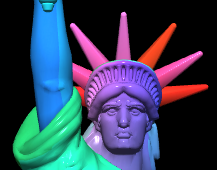
\includegraphics[width=\textwidth]{images/HeadManualWithoutSnow.png}
      \caption{First image caption}
      \label{fig:image1}
  \end{minipage}\hfill
  \begin{minipage}{0.45\textwidth}
      \centering
      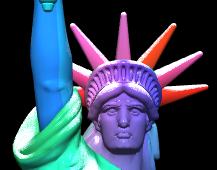
\includegraphics[width=\textwidth]{images/HeadManualWithSnow.png}
      \caption{Second image caption}
      \label{fig:image2}
  \end{minipage}
\end{figure}



\subsubsection {Full Snow Equation}

\subsection {Environment Simulation}

%  Environment 1: Temperature
\subsubsection {Temperature}
The temperature of a location depends on multiple factors, e.g., time of the day, season, altitude, 
latitude and distance to the ocean. To create a reasonable snow effect, the location used in this paper 
is an in-land city around the latitude of 35$^{\circ}$ N or 35$^{\circ}$ S and the season is winter.

This location has a large temperature difference. The highest temperature is about 
\(10^\circ\mathrm{C}\), which can be reached at around 1-2 P.M. The lowest temperature is about 
\(-10^\circ\mathrm{C}\), which can be reached at around 5-7 A.M. The hourly temperature data can be
obtained on weather forecast websites, and the Cubic Spline method is used to interpolate the 
intermediate values, making the temperature-time curve smoother.

%  Environment 2: Snow Factor
\subsubsection {Snow Factor}
The snow factor is the user-defined function \( f_{u}(p) \) in Section TODO:1, causing a potentially 
negative effect on the original snow. The range is between 0 and 1, where 0 means that the snow is 
disabled regardless of the original snow, and 1 means that there are no negative effects.
To simplify the simulation, the snow factor is based solely on the environmental temperature. 

If the temperature is below or equal to \(0^\circ\mathrm{C}\), the snow factor is always 1. 
If the temperature is above or equal to \(5^\circ\mathrm{C}\), the snow factor is always 0. 
Otherwise, the snow factor decreases linearly from 1 to 0 as temperature increases.

\[
  f_{u}(p)=
  \left\{
    \begin{array}{ll}
      0 & t\leq 0 \\
      1 - \frac{t}{5} &  0 < t < 5 \\
      1 & t\geq 5 \\
    \end{array} 
  \right. 
\]
\text{where } t \text{ is the temperature in degrees Celsius.}

% The following figures are temperature - time relationship and snow amount - time relationship

\begin{figure}[h]
  \centering
  \begin{minipage}{0.45\textwidth}
      \centering
      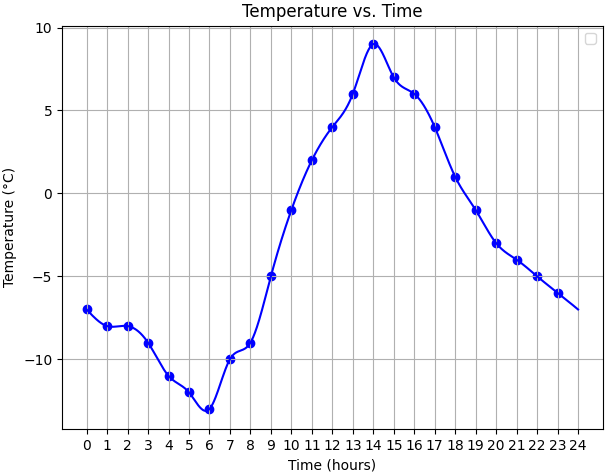
\includegraphics[width=\textwidth]{images/Temperature35N.png}
      \caption{Temperature throughout the day}
      \label{fig:Temperature35N}
  \end{minipage}\hfill
  \begin{minipage}{0.45\textwidth}
      \centering
      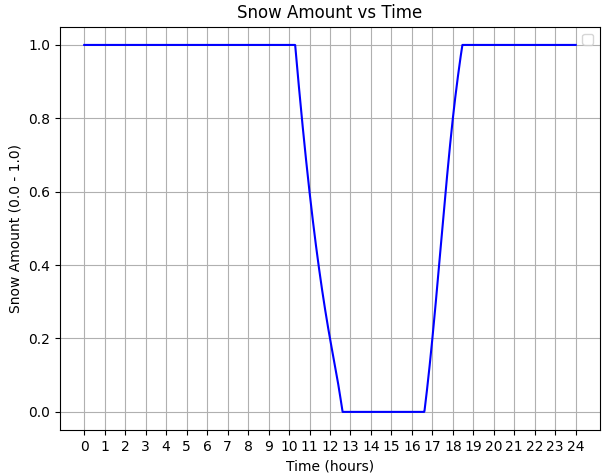
\includegraphics[width=\textwidth]{images/SnowAmount35N.png}
      \caption{Snow amount throughout the day}
      \label{fig:SnowAmount35N}
  \end{minipage}
\end{figure}

%  Environment 3: Sunlight Intensity
\subsubsection {Sunlight Intensity}
In the real world, there are multiple light sources outside, including the sun, sky, moon, stars, 
and human-made lights. In this paper, only the sunlight and sky (ambient) light are considered. 
The intensity of the skylight is a small constant value while that of the sunlight varies by 
time, ranging from 0 to 1.

Assume the light intensity of the sun is 0 (or a very small value) at night. It starts increasing 
rapidly (typically 30 minutes) before sunrise and reaches the maximum value in a short time 
(typically 1-3 hours). It remains stable until several hours before the sunset. The value 
decreases quickly in the sunset period and finally returns to 0 (or a very small value). Here is 
the mathematical formula of the light intensity.

\[
  I = e^{-\frac{\left(\frac{\pi}{2} - \theta\right)^{\frac{m}{60} + 1}}{b}}
\]

where:
\begin{itemize}
  \item \( I \) is the light intensity of the simulated sun, \( I \in (0, 1] \).
  \item \( \theta \) is the solar elevation angle in radians, which is based on the current time, 
  season (declination) and position (latitude).
  \item \( m \) is the total daylight time (in minutes) in that day, \( m \in [0, 1440) \), \( m \in \mathbb{Z} \). 
  For example, if the sunrise time is 6 AM and the sunset time is 6 PM, \( m=720 \) (12 hours)
  \item \( b \) is a bias factor adjusting the exponent decay rate, making the light intensity
  transition more realistic.
\end{itemize}

The bias \( b \) depends on multiple factors, including the altitude, latitude and time zone. To
simplify the simulation, it can be calculated by solving an equation in terms of \( m \) when 
\( I \) and \( \theta\) is given.

\[
  b = -\frac{\left(\frac{\pi}{2} - \theta\right)^{\frac{m}{60} + 1}}{\log(I)}
\]

Assume the solar light intensity is 0.1 on sunrise or sunset (i.e., \( \theta=0\)), the formula 
of the bias can be expressed as:

\[
  b = \frac{\left(\frac{\pi}{2}\right)^{\frac{m}{60} + 1}}{\log(10)}
\]

\begin{figure}[h]
  \centering
  \begin{minipage}{0.45\textwidth}
      \centering
      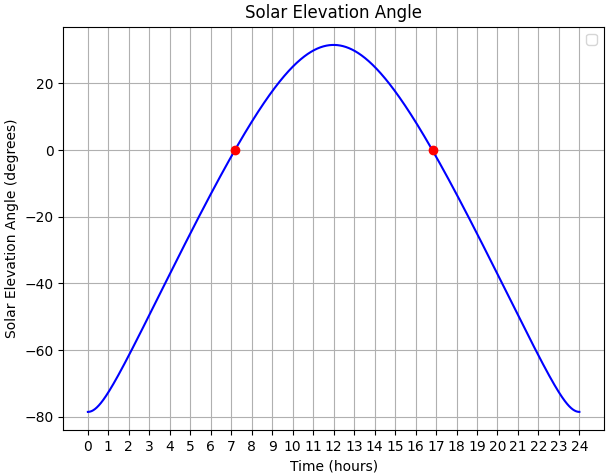
\includegraphics[width=\textwidth]{images/SolarElevetion35N.png}
      \caption{Solar elevation angle throughout the day}
      \label{fig:SolarElevetion35N}
  \end{minipage}\hfill
  \begin{minipage}{0.45\textwidth}
      \centering
      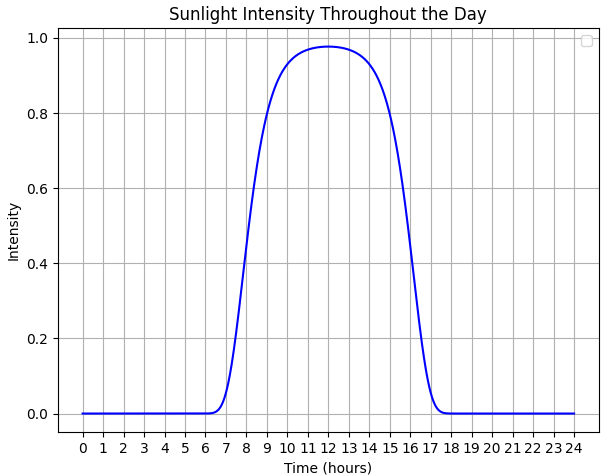
\includegraphics[width=\textwidth]{images/SunlightIntensity35N.png}
      \caption{Sunlight intensity throughout the day}
      \label{fig:SunlightIntensity35N}
  \end{minipage}
\end{figure}

% TODO: Sunlight direction

%  Environment 4: Sunlight and Sky Color
\subsubsection {Sunlight and Sky Color}
Sunlight and sky colors depend on the current time. Typically on a sunny day, the sunlight is yellow
to white for most of the day and it becomes orange during sunrise or sunset. The sky is light blue
in the day, orange during sunrise or sunset and dark purple at night. To simulate those colors, 
interpolation is also needed to make the transition process smoother. 

\[
  C_{b}=
  \left\{
    \begin{array}{ll}
      \text{night} & \theta \leq 10 \\
      \text{interpolate(night, twilight)} &  -10 \leq t < 5 \\
      \text{interpolate(twilight, day)} &  5 \leq t < 20 \\
      \text{day} & t \geq 20 \\
    \end{array} 
  \right. 
\]




\begin{figure}[h]
  \centering
  \begin{minipage}{0.45\textwidth}
      \centering
      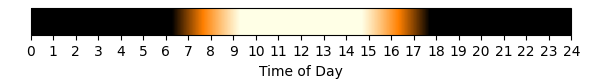
\includegraphics[width=\textwidth]{images/SunColor35N.png}
      \caption{First image caption}
      \label{fig:SunColor35N}
  \end{minipage}\hfill
  \begin{minipage}{0.45\textwidth}
      \centering
      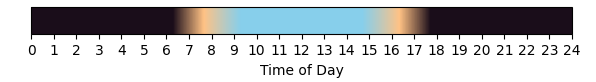
\includegraphics[width=\textwidth]{images/SkyColor35N.png}
      \caption{Second image caption}
      \label{fig:SkyColor35N}
  \end{minipage}
\end{figure}


\section{Experiments and Results}

% Result 1: Pure Snow Effect
\subsection {Pure Snow Effect}
The following figure group is the rendering effect with full snow, half snow, and no snow respectively.
The dynamic environment system is disabled and the light source is always right above the object with
the maximum intensity and white color. Those three sub-figures illustrate the effect on both declination 
(the head and book of the statue) and occlusion (the feet area of it), as well as the color blending
mentioned above.

\begin{figure}[h]
  \centering
  \subfloat[Snow Amount = 0.0]{
    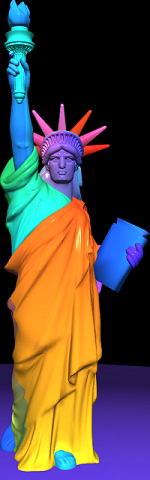
\includegraphics[width=0.30\textwidth]{images/AllTimeNaNNoSnow.png}
    \label{fig:AllTimeNaNNoSnow}
  }\hfill
  \subfloat[Snow Amount = 0.5]{
    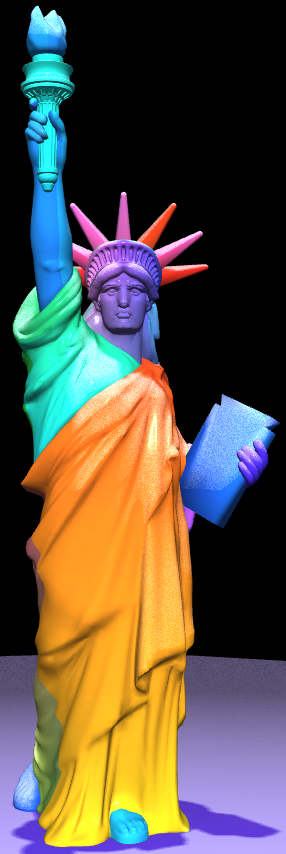
\includegraphics[width=0.30\textwidth]{images/AllTimeNaNHalfSnow.png}
    \label{fig:AllTimeNaNHalfSnow}
  }\hfill
  \subfloat[Snow Amount = 1.0]{
    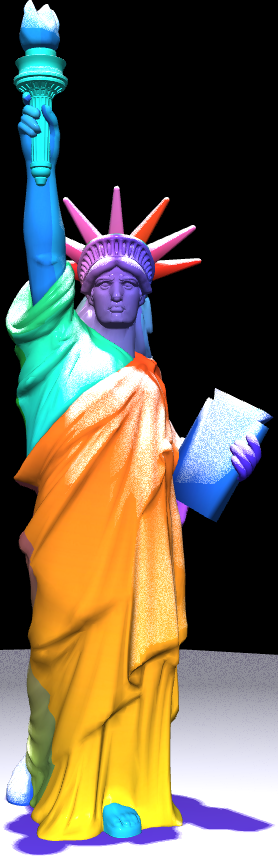
\includegraphics[width=0.30\textwidth]{images/AllTimeNaNFullSnow.png}
    \label{fig:AllTimeNaNFullSnow}
  }
  \caption{Object covered by different amounts of snow}
  \label{fig:9}
\end{figure}

% Result 2: Snow Effect with Dynamic Daylight Simulation
\subsection {Snow Effect with Dynamic Daylight Simulation}
\label{headings}
The following figure group is the rendering effect at different times with the location and season mentioned 
above (35 $^{\circ}$S on June \(22^{nd}\)). The sunrise time is about 7 AM and the sunset time is about 5 PM.

Throughout the night (e.g., midnight (a) or 7:00 PM (f)), the temperature is quite low and the sunlight 
intensity is almost zero so the object is fully covered by white snow and only ambient colors can be seen. The
sky color should be very dark.

In the morning (e.g., 8:00 AM (b)), the sunlight intensity increases with an orange color, resulting in a yellow
snow color and an orange sky color. The snow coverage is still 100 \% as the temperature is still below 
\(0^\circ\mathrm{C}\). Around noon (e.g., 11:00 AM (c)), the sky becomes light blue and the snow color becomes 
back to white as the sunlight color is pretty white. The snow starts melting at this time so part of the covered 
object can be seen now. 

In the afternoon (e.g., 2:00 PM (d)), the weather is warmest. As a result, there is no snow on the scene. During 
the sunset period, (e.g., 5:00 PM (e)), the sunlight intensity drops back and the sunlight color / sky color becomes
orange again. The snow effect is back due to the dropping temperature.

\begin{figure}[h]
  \centering
  \subfloat[Time = 12:00 AM]{
    \includegraphics[width=0.3\textwidth]{images/AllT0000L35S.png}
    \label{fig:AllT0000L35S}
  }\hfill
  \subfloat[Time = 08:00 AM]{
    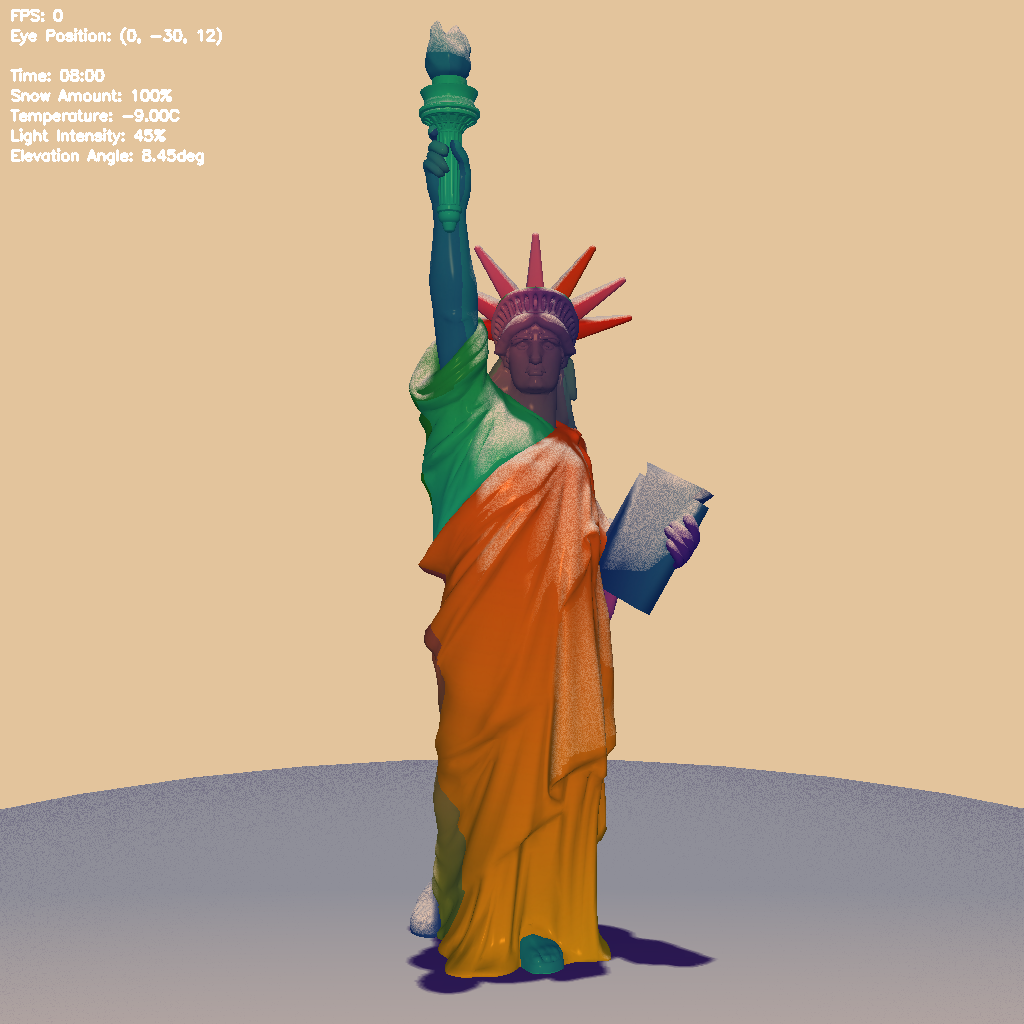
\includegraphics[width=0.3\textwidth]{images/ALLT0800L35S.png}
    \label{fig:ALLT0800L35S}
  }\hfill
  \subfloat[Time = 11:00 AM]{
    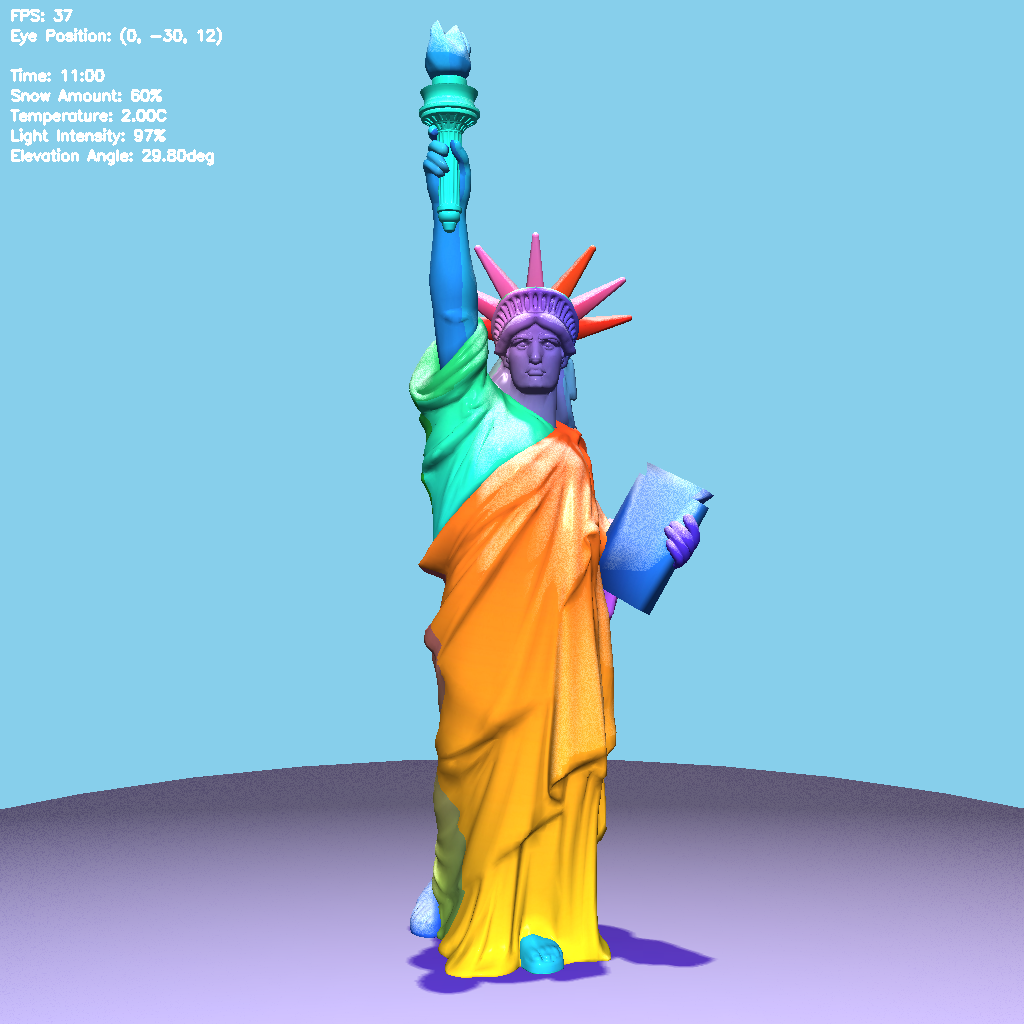
\includegraphics[width=0.3\textwidth]{images/ALLT1100L35S.png}
    \label{fig:ALLT1100L35S}
  }

  \subfloat[Time = 02:00 PM]{
    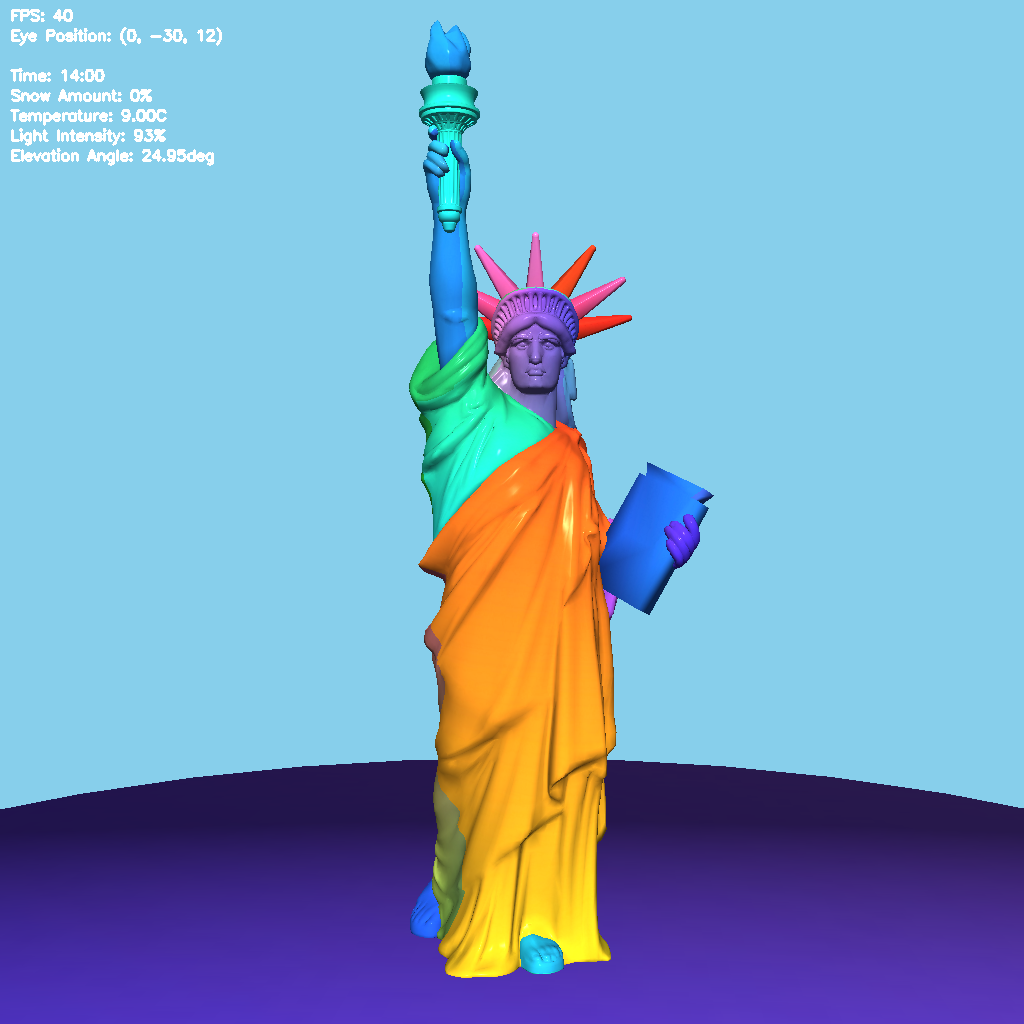
\includegraphics[width=0.3\textwidth]{images/ALLT1400L35S.png}
    \label{fig:ALLT1400L35S}
  }\hfill
  \subfloat[Time = 05:00 PM]{
    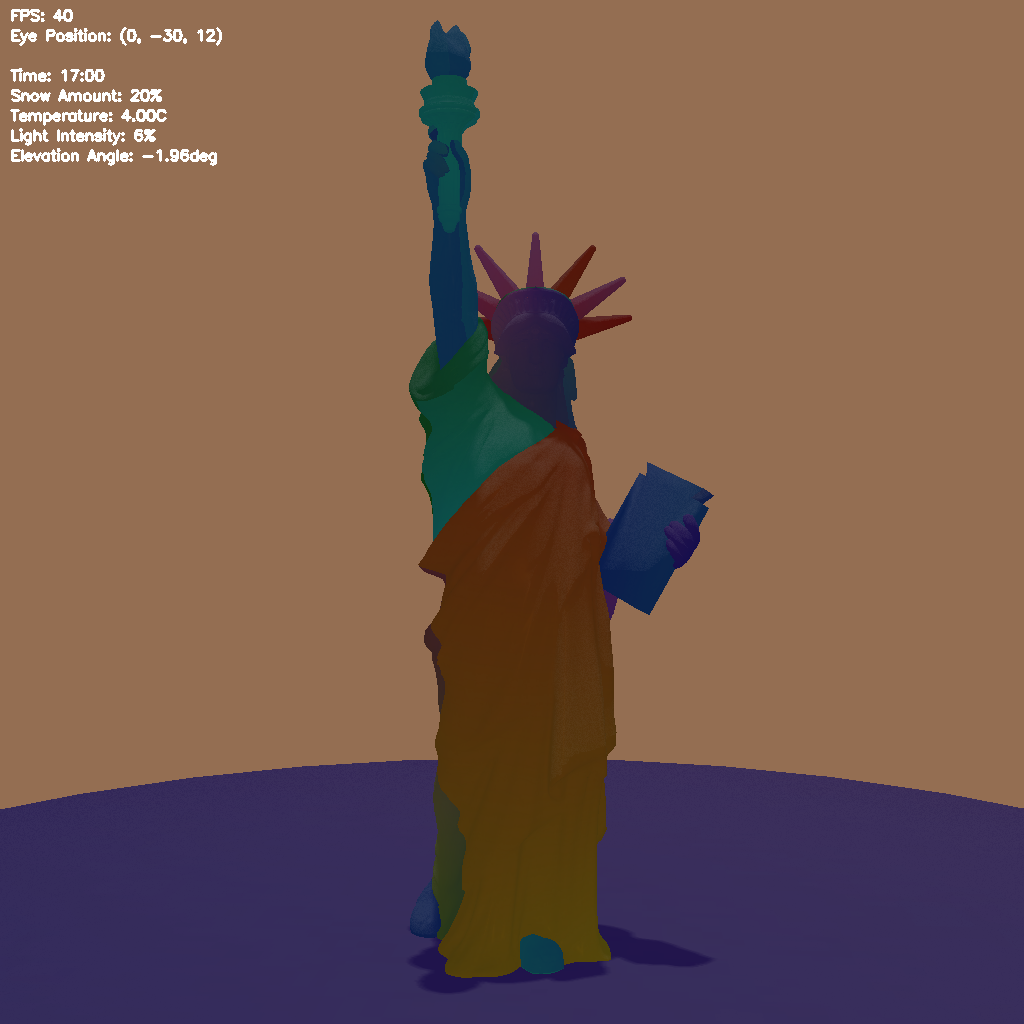
\includegraphics[width=0.3\textwidth]{images/ALLT1700L35S.png}
    \label{fig:ALLT1700L35S}
  }\hfill
  \subfloat[Time = 07:00 PM]{
    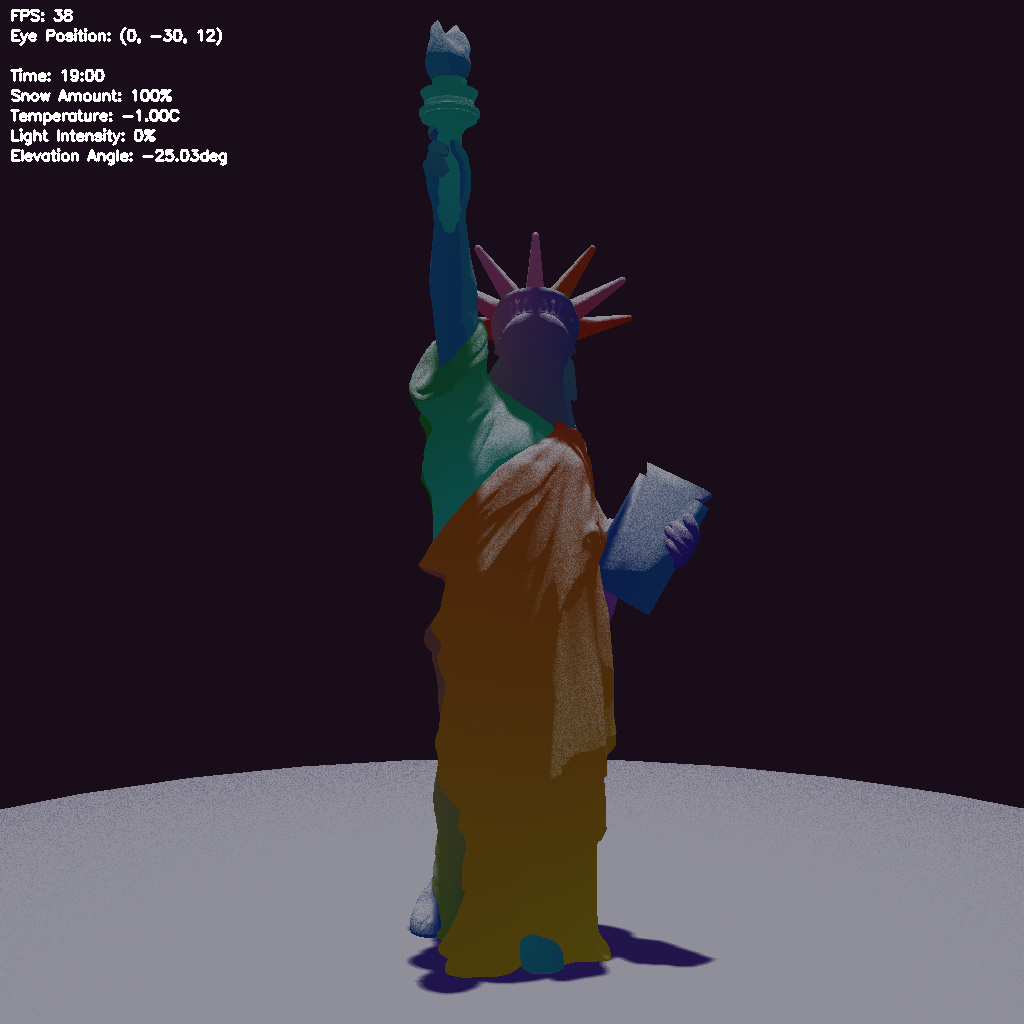
\includegraphics[width=0.3\textwidth]{images/ALLT1900L35S.png}
    \label{fig:ALLT1900L35S}
  }

  \caption{The rendered scene in different time (at 35 $^{\circ}$S on June \(22^{nd}\))}
  \label{fig:AllL35S}
\end{figure}

The following figure group is the plot of the data at different times with a high latitude location on the summer 
solstice (60 $^{\circ}$N on June \(22^{nd}\)). The sunrise time is about 2:30 AM and the sunset time is about 9:30 
PM, so there are 19 hours of daylight time.

\begin{figure}[h]
  \centering
  \subfloat[Time = s]{
    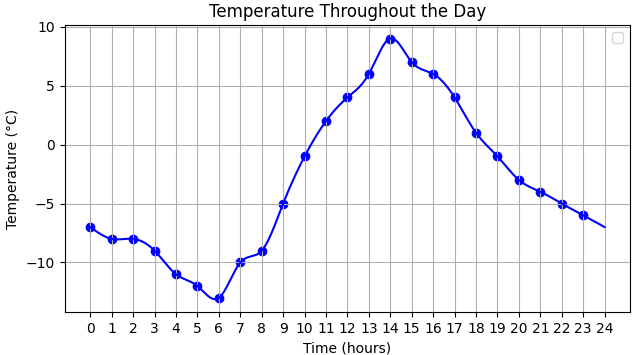
\includegraphics[width=0.3\textwidth]{images/Temperature60N.png}
    \label{fig:image111}
  }\hfill
  \subfloat[Time = 8 AM]{
    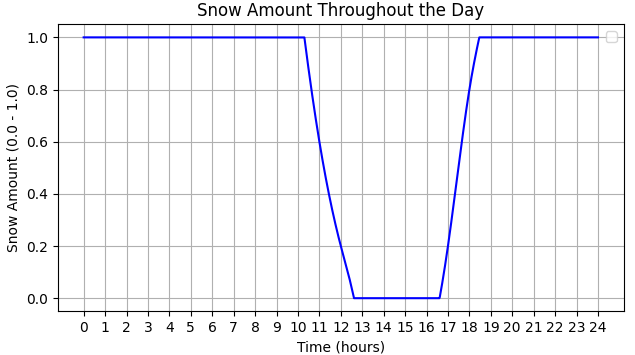
\includegraphics[width=0.3\textwidth]{images/SnowAmount60N.png}
    \label{fig:image222}
  }\hfill
  \subfloat[Time = 10 AM]{
    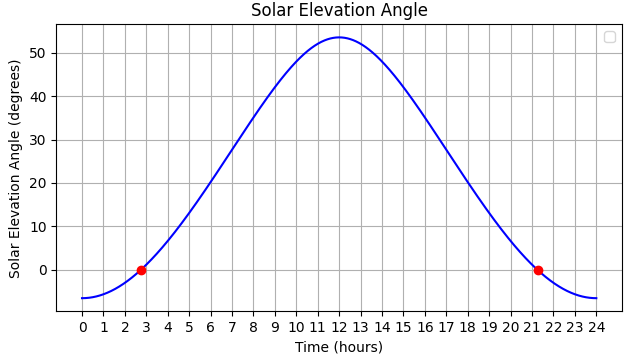
\includegraphics[width=0.3\textwidth]{images/SolarElevetion60N.png}
    \label{fig:image333}
  }

  \subfloat[Time = 11 AM]{
    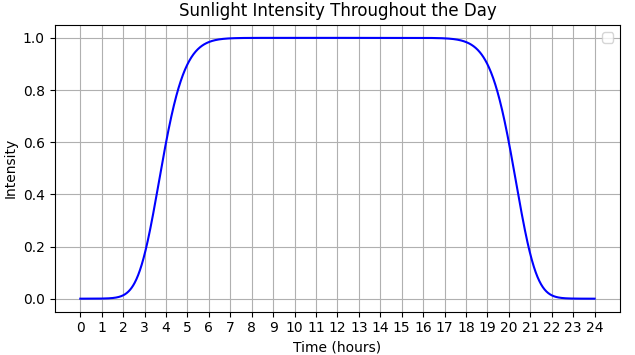
\includegraphics[width=0.3\textwidth]{images/SunlightIntensity60N.png}
    \label{fig:image444}
  }\hfill
  \subfloat[Time = 2 PM]{
    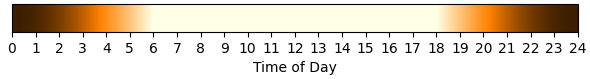
\includegraphics[width=0.3\textwidth]{images/SunColor60N.png}
    \label{fig:image555}
  }\hfill
  \subfloat[Time = 5 PM]{
    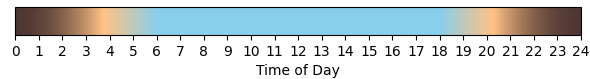
\includegraphics[width=0.3\textwidth]{images/SkyColor60N.png}
    \label{fig:image666}
  }

  \caption{The rendered scene in different time}
  \label{fig:mainfigure123}
\end{figure}

The following figure group is the rendering effect in the above location. In the summer of the high-latitude locations,
each day has a long daylight time. Throughout the night (e.g., midnight (a)), the sky is not completely dark even if
the sun is below the horizon. 

At 8:00 AM (b), the sunlight intensity has already reached the maximum value. The scenes between the two locations are 
similar during the noon or afternoon time (c or d), except for the solar position. However, because of the high latitude,
the sunlight intensity keeps the high value at 5:00 PM (e) and finally starts dropping at around 7:00 PM (f).

\begin{figure}[h]
  \centering
  \subfloat[Time = 12:00 AM]{
    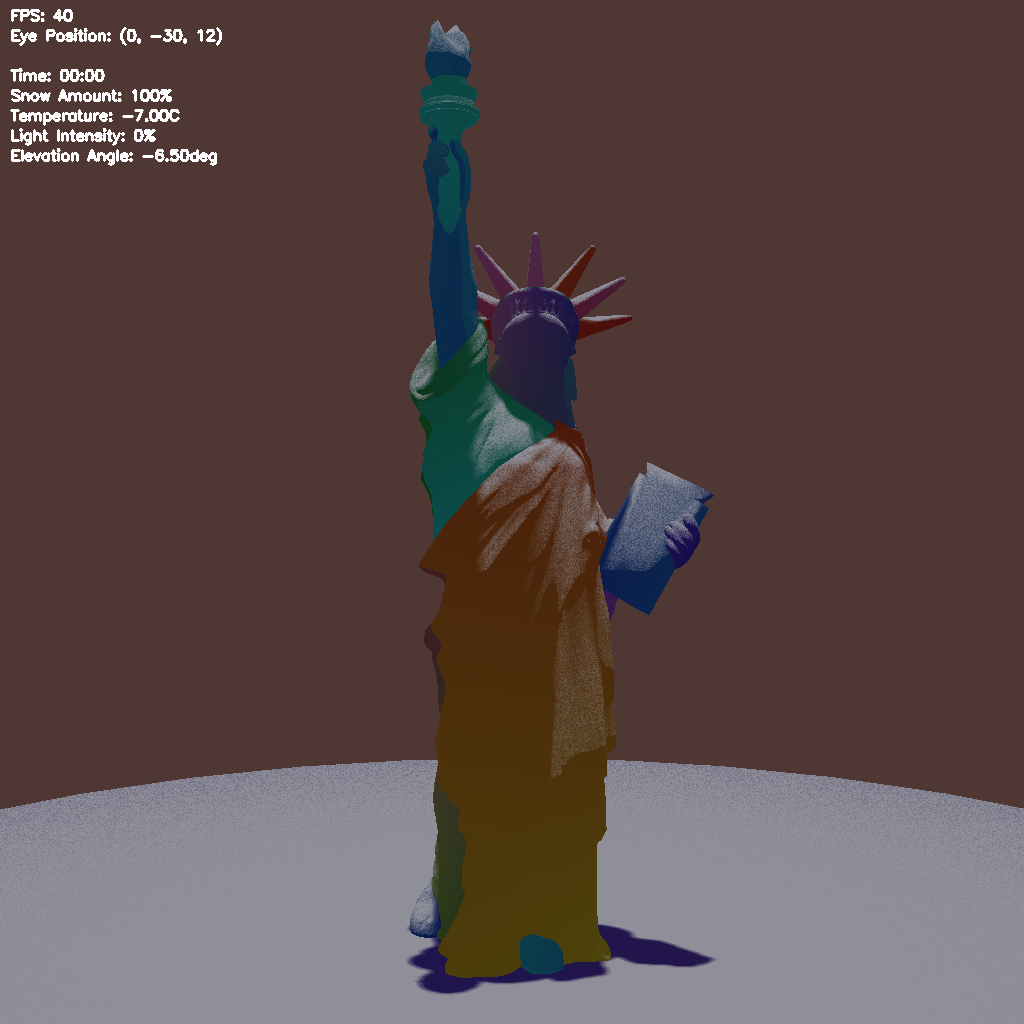
\includegraphics[width=0.3\textwidth]{images/ALLT0000L60N.png}
    \label{fig:ALLT0000L60N}
  }\hfill
  \subfloat[Time = 08:00 AM]{
    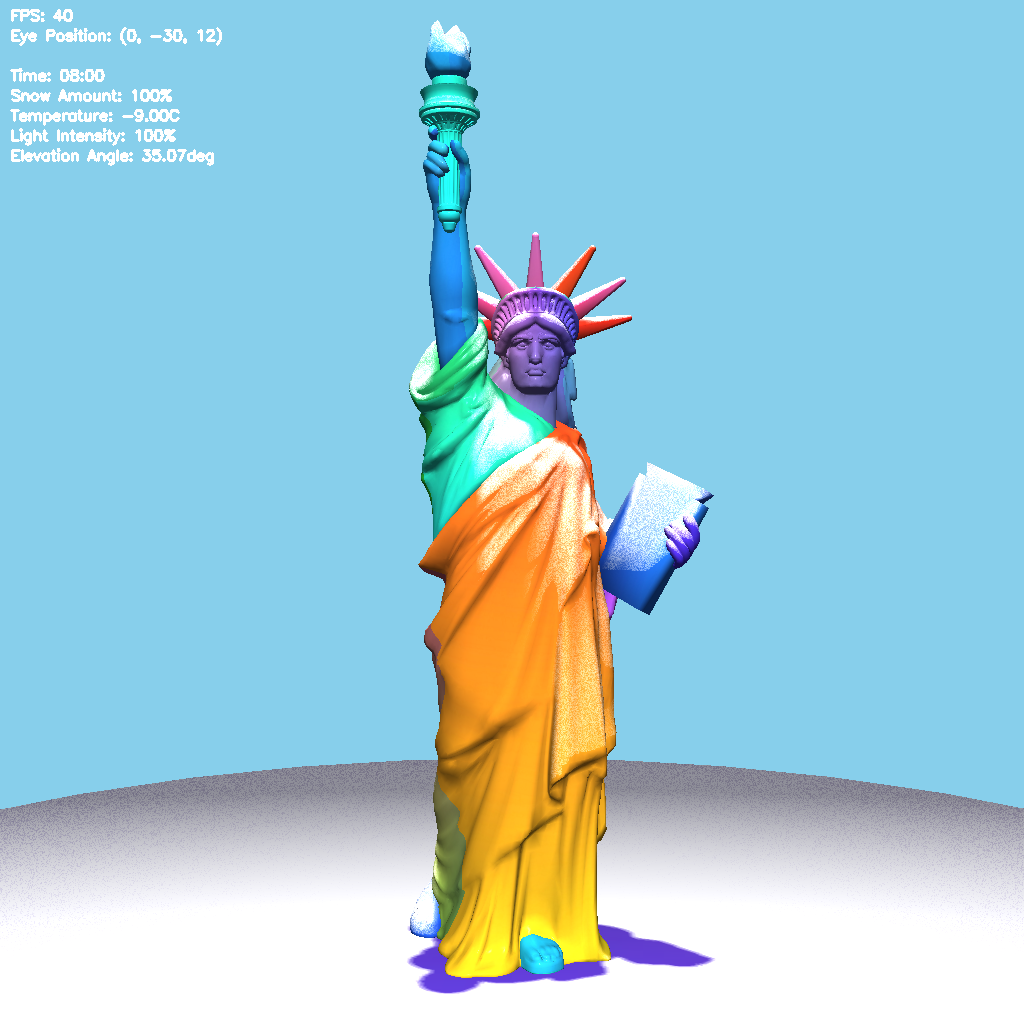
\includegraphics[width=0.3\textwidth]{images/ALLT0800L60N.png}
    \label{fig:ALLT0800L60N}
  }\hfill
  \subfloat[Time = 11:00 AM]{
    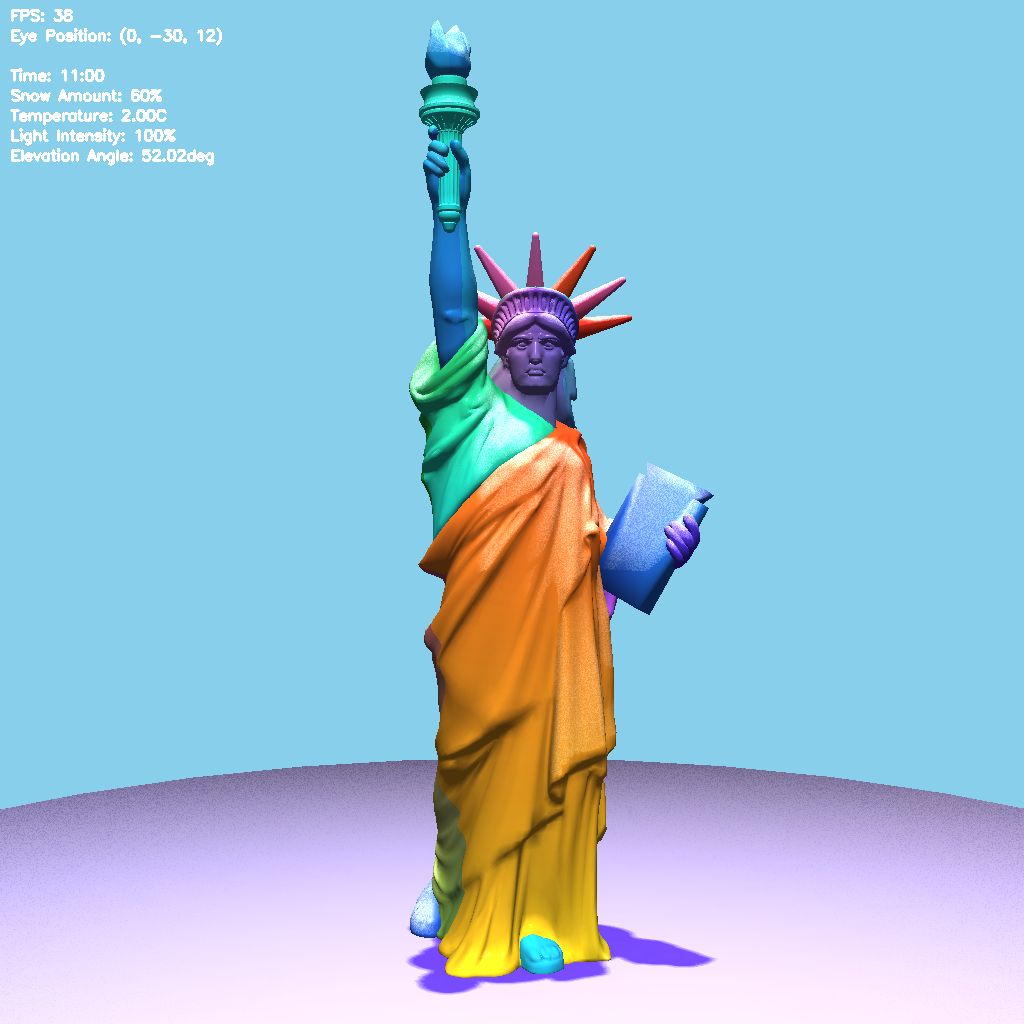
\includegraphics[width=0.3\textwidth]{images/ALLT1100L60N.png}
    \label{fig:ALLT1100L60N}
  }
  
  \subfloat[Time = 02:00 PM]{
    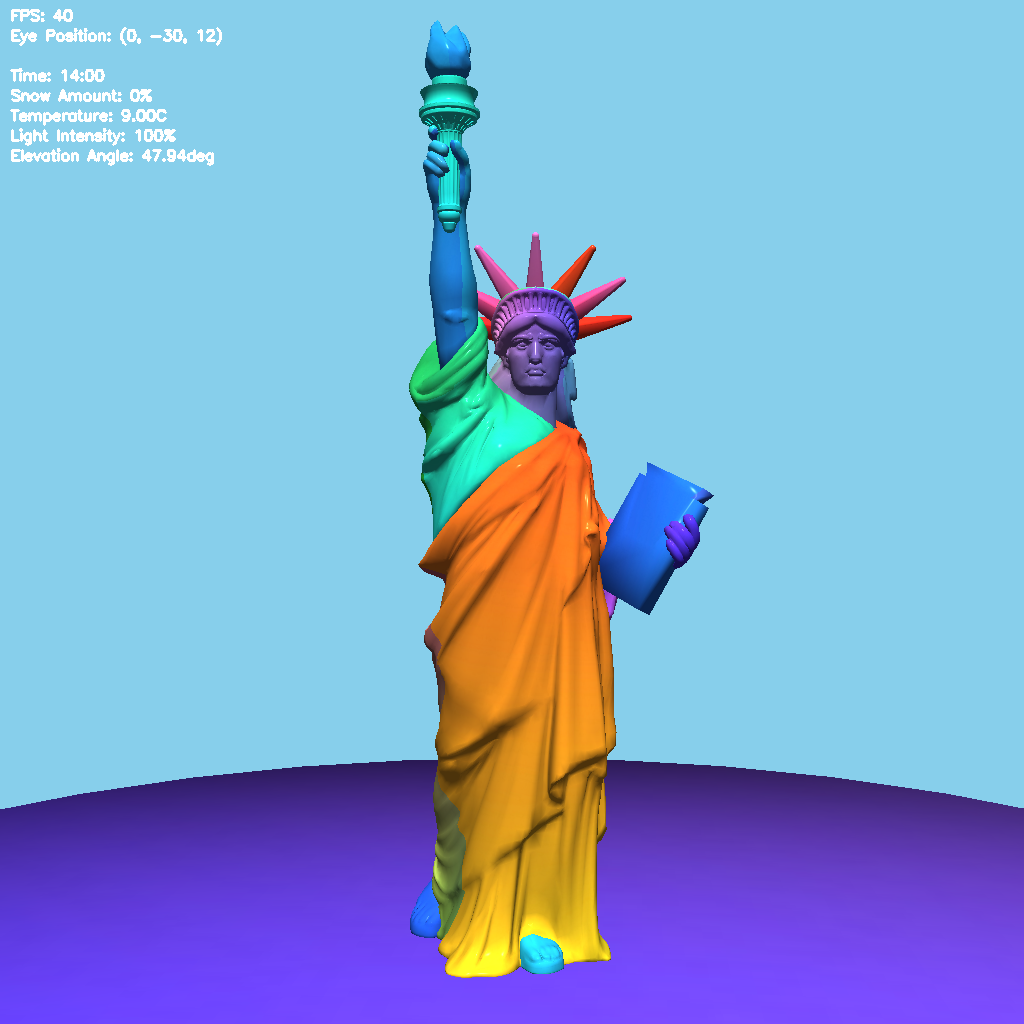
\includegraphics[width=0.3\textwidth]{images/ALLT1400L60N.png}
    \label{fig:ALLT1400L60N}
  }\hfill
  \subfloat[Time = 05:00 PM]{
    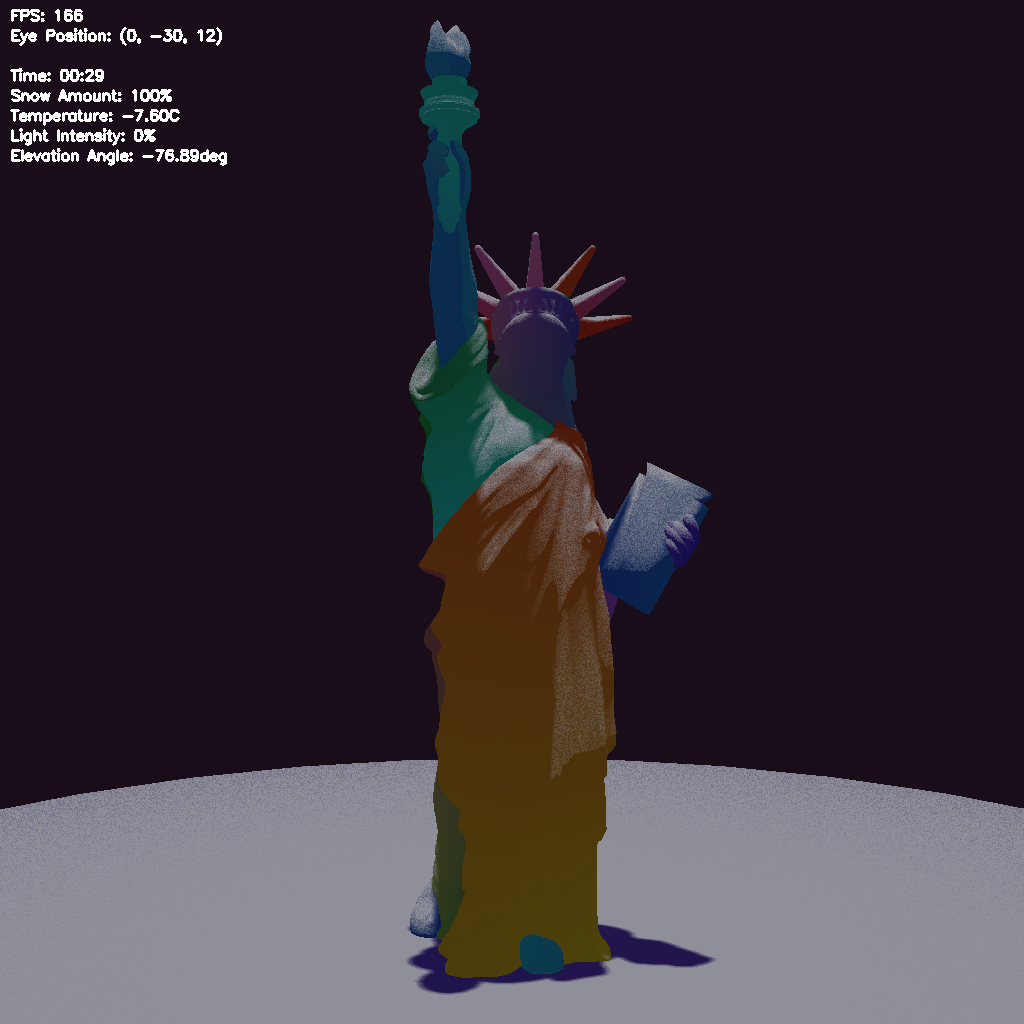
\includegraphics[width=0.3\textwidth]{images/ALLT1700L60N.png}
    \label{fig:ALLT1700L60N}
  }\hfill
  \subfloat[Time = 07:00 PM]{
    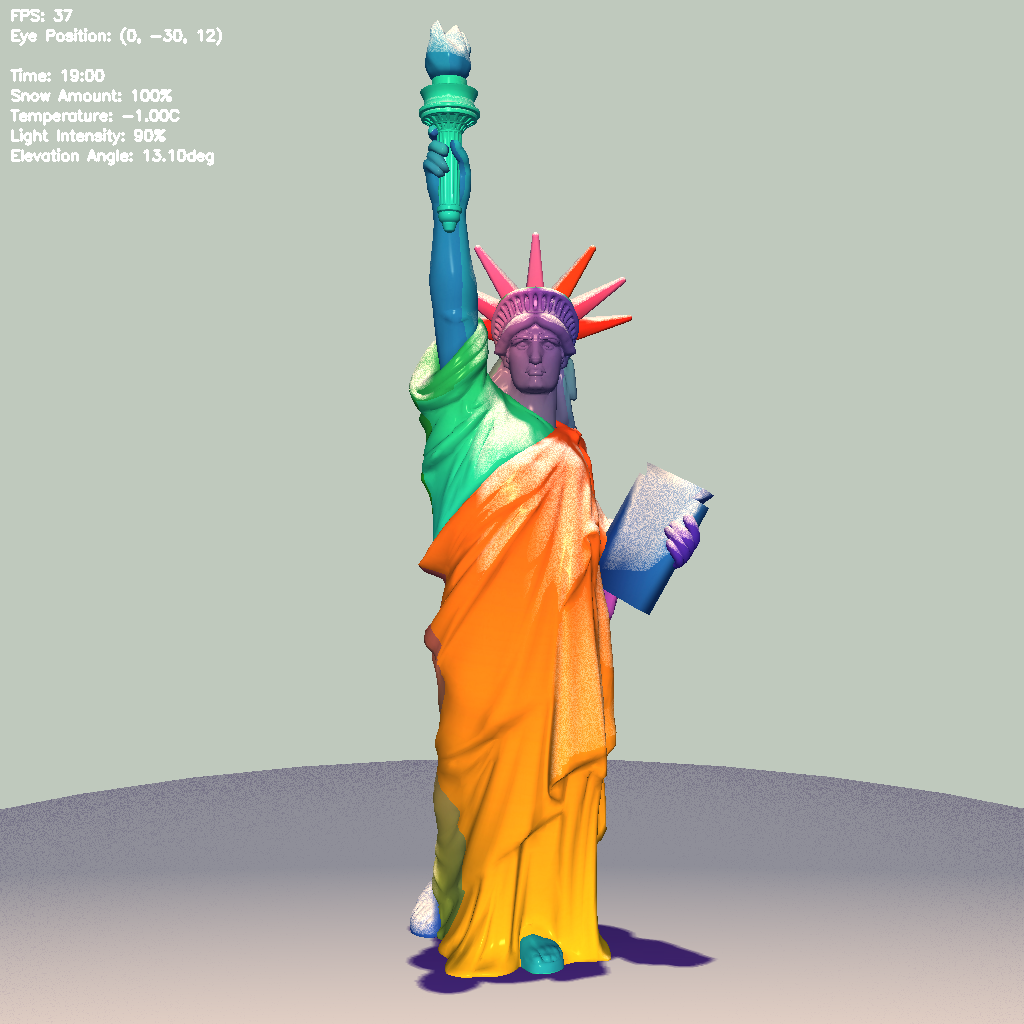
\includegraphics[width=0.3\textwidth]{images/ALLT1900L60N.png}
    \label{fig:ALLT1900L60N}
  }

  \caption{The rendered scene in different time (at 60 $^{\circ}$N on June \(22^{nd}\))}
  \label{fig:AllL60N}
\end{figure}

\section{Discussions and Conclusion}
Please prepare submission files with paper size ``US Letter,'' and not, for
example, ``A4.''


Fonts were the main cause of problems in the past years. Your PDF file must only
contain Type 1 or Embedded TrueType fonts. Here are a few instructions to
achieve this.


\section*{References}

{
\small


[1] Alexander, J.A.\ \& Mozer, M.C.\ (1995) Template-based algorithms for
connectionist rule extraction. In G.\ Tesauro, D.S.\ Touretzky and T.K.\ Leen
(eds.), {\it Advances in Neural Information Processing Systems 7},
pp.\ 609--616. Cambridge, MA: MIT Press.


[2] Bower, J.M.\ \& Beeman, D.\ (1995) {\it The Book of GENESIS: Exploring
  Realistic Neural Models with the GEneral NEural SImulation System.}  New York:
TELOS/Springer--Verlag.


[3] Hasselmo, M.E., Schnell, E.\ \& Barkai, E.\ (1995) Dynamics of learning and
recall at excitatory recurrent synapses and cholinergic modulation in rat
hippocampal region CA3. {\it Journal of Neuroscience} {\bf 15}(7):5249-5262.
}

\section*{Additional Experiment Results}

\section*{Confidential Peer Review} 

The percentage, who did what, ratio weights. 






\end{document}